%% ======================================================================
%% 03_description.tex -- 2. Descripcion del hardware (arquitectura, alimentacion, pines, decisiones)
%% ======================================================================
\section{Descripción del hardware}
\label{sec:description}

\subsection{Arquitectura}
La Fig.~\ref{fig:overview} muestra el prototipo final y su modelo CAD, y la Fig.~\ref{fig:architecture} su arquitectura eléctrica y de comunicaciones. El robot se organiza en cuatro subsistemas (tres niveles mecánicos y la electrónica auxiliar):

\begin{figure}[!htbp]
  \centering
  \begin{subfigure}[b]{0.43\textwidth}\centering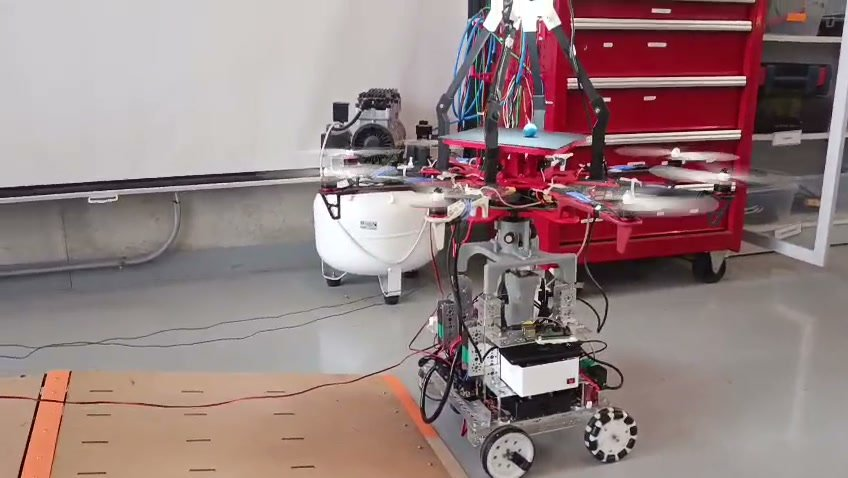
\includegraphics[width=\linewidth]{figures/photo_robot_side.jpg}\caption{Prototipo integrado.}\end{subfigure}\hfill
  \begin{subfigure}[b]{0.30\textwidth}\centering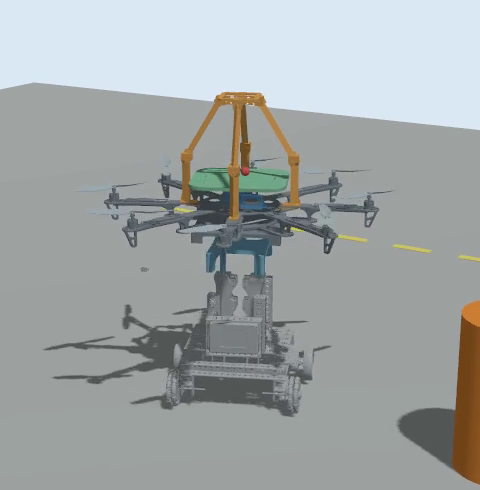
\includegraphics[width=\linewidth]{figures/cad_assembly.png}\caption{Ensamble CAD (383 piezas).}\end{subfigure}\hfill
  \begin{subfigure}[b]{0.25\textwidth}\centering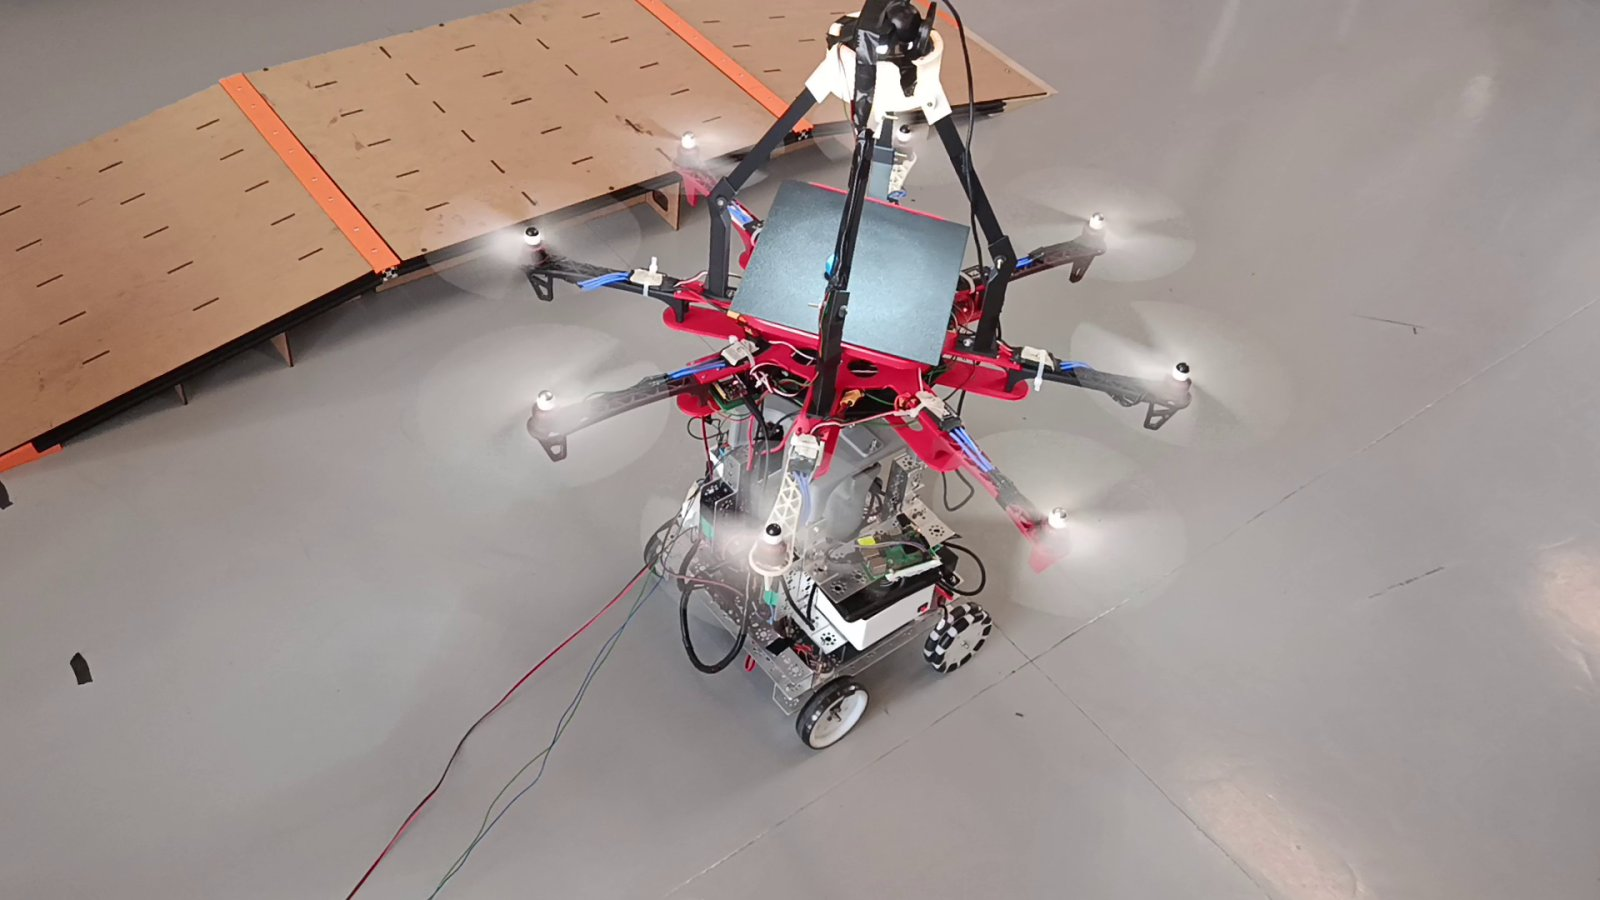
\includegraphics[width=\linewidth,trim=420 0 420 0,clip]{figures/photo_ramp_top.jpg}\caption{Sobre la rampa de \SI{10}{\degree}.}\end{subfigure}
  \caption{AeroTray. De abajo hacia arriba: base diferencial TETRIX con la myRIO, mástil con guía vertical, rótula esférica, octocóptero (marco rojo, ocho rotores) y bandeja del \textit{ball and plate} con la cámara cenital. La bola azul tiene \SI{27}{\milli\metre} de diámetro.}
  \label{fig:overview}
\end{figure}

\begin{enumerate}[label=\textbf{N\arabic*.}]
  \item \textbf{Base móvil.} Chasis de aluminio TETRIX MAX con dos ruedas motrices (motores DC TETRIX TorqueNADO con encoders en cuadratura) y dos ruedas omnidireccionales como apoyos pasivos. Una NI myRIO-1900 lee los encoders, calcula la odometría y ejecuta un lazo PI de velocidad por rueda; un puente H MDD10A alimenta los motores desde una batería NiMH TETRIX de \SI{12}{\volt}. Trocha $b=\SI{0.3794}{\metre}$; avance de la rueda por cuenta de encoder \SI{0.2151}{\milli\metre} (radio de rueda $r\approx\SI{49.3}{\milli\metre}$).
  \item \textbf{Módulo aéreo.} Octocóptero con brazos de radio $L=\SI{0.350}{\metre}$ (un motor cada \SI{45}{\degree}), ocho motores sin escobillas A2212 de 920\,KV con hélices 9450 y ESC de 30\,A sin BEC, dos baterías LiPo 3S de \SI{3300}{\milli\ampere\hour} (una por cada grupo de cuatro ESC), una IMU MPU-6050 y un sensor de tiempo de vuelo VL53L0X que mide la distancia a un blanco blanco mate fijo en la base (Sección~\ref{sec:altura}). Una NodeMCU-32S (ESP32) ejecuta el control de actitud a \SI{200}{\hertz}. El módulo se une al mástil mediante una rótula esférica montada en un carro que desliza por una guía vertical (recorrido medido de unos \SI{140}{\milli\metre}); la rótula deja libres el alabeo y el cabeceo y, por su fricción y sus topes, solo permite un giro pequeño de guiñada, de modo que el octocóptero gira con la base. El conjunto móvil pesa \SI{3.6}{\kilo\gram} (\SI{3.3}{\kilo\gram} el conjunto que rota y \SI{0.3}{\kilo\gram} el carro). El plano de los rotores está \SI{95}{\milli\metre} sobre el centro de la rótula.
  \item \textbf{Bandeja del \textit{ball and plate}.} Plato de $\SI{250}{\milli\metre}\times\SI{220}{\milli\metre}$ apoyado en su centro sobre una junta universal (cruceta) en un pilar fijo a la placa central del octocóptero, \SI{104}{\milli\metre} sobre la rótula, e inclinado en dos ejes por dos servos Futaba S3003 mediante mecanismos de cuatro barras (Sección~\ref{sec:linkage}). Una ESP32-S3 genera los pulsos de \SI{50}{\hertz} de los servos (GPIO47 para $x$, GPIO21 para $y$) y ejecuta el PID de la bola. Una cámara PS3 Eye, sostenida a $\approx$\SI{0.20}{\metre} sobre el plato por cuatro torres fijas al octocóptero (no al plato), envía cuadros de $320\times240$ a \SI{187}{fps} a la Raspberry Pi, que detecta la bola y envía su posición y velocidad a la ESP32-S3.
  \item \textbf{Supervisor, distribución electrónica y paro.} La Raspberry Pi 3B+ centraliza la visión, los enlaces y el registro, con dominios separados de lógica y paro de emergencia (Sección~\ref{sec:power}). En el módulo aéreo, las dos controladoras van debajo de la placa central, en brazos opuestos, para repartir el peso y separar el ruido de los ESC: la NodeMCU-32S (control de actitud) en el brazo 8 ($+x$) y la ESP32-S3 (bandeja) en el brazo 6 ($-x$). La IMU MPU-6050 y el láser VL53L0X están junto a la NodeMCU en el brazo 8, en el mismo bus I$^2$C. El láser apunta hacia abajo, al blanco fijo en la base. Por eso ambos sensores están desplazados del eje de la rótula, y la Sección~\ref{sec:altura} corrige la medida de altura por ese brazo de palanca.
\end{enumerate}

\begin{figure}[!htbp]
\centering
\begin{tikzpicture}[font=\footnotesize, >=Latex,
  colhdr/.style={font=\footnotesize\bfseries, text=pGris!85!black, align=center},
  blk/.style={draw, rounded corners=2pt, align=center, minimum height=11.5mm, inner xsep=2pt, inner ysep=2.5pt, line width=0.6pt},
  blkusr/.style={blk, fill=white, draw=pGris, text width=3.34cm},
  blkpw/.style={blk, fill=pRojo!7, draw=pRojo, text width=3.34cm},
  blkcp/.style={blk, fill=pAzul!7, draw=pAzul, text width=3.34cm},
  blksa/.style={blk, fill=pVerde!7, draw=pVerde, text width=4.04cm},
  pw/.style={->, line width=1.05pt, pRojo, rounded corners=2pt},
  pwbr/.style={pw, preaction={-, draw=white, line width=2.6pt, rounded corners=2pt}},
  dt/.style={<->, line width=0.85pt, pAzul, rounded corners=2pt},
  dt1/.style={->, line width=0.85pt, pAzul, rounded corners=2pt},
  lab/.style={font=\footnotesize, text=pAzul!90!black, inner sep=1.5pt}]
  % Coordenadas de las 3 columnas (ancho total = 13.38 cm < 13.74 cm = \textwidth)
  % Col 1: x=1.74 ([0.00, 3.48]), Col 2: x=6.28 ([4.54, 8.02]), Col 3: x=11.24 ([9.15, 13.33])
  \node[colhdr] at (1.74, -0.84) {Alimentación};
  \node[colhdr] at (6.28, 0.90) {Cómputo};
  \node[colhdr] at (11.24, 0.90) {Sensores y actuadores};

  % ---- Fila 1 (y = 0.00) -- todas las cajas de exactamente 2 lineas y mismo alto
  \node[blkusr] (web)  at (1.74,  0.00) {\textbf{Navegador}\\ laptop o celular};
  \node[blkcp]  (pi)   at (6.28,  0.00) {\textbf{Raspberry Pi 3B+}\\ visión, registro y web};
  \node[blksa]  (cam)  at (11.24, 0.00) {\textbf{Cámara PS3 Eye}\\ 320$\times$240 a 187 fps};

  % ---- Fila 2 (y = -1.68)
  \node[blkpw]  (pipw) at (1.74, -1.68) {\textbf{BT5: 3S 18650}\\ XL4015 $\to$ 5,2 V};
  \node[blkcp]  (s3)   at (6.28, -1.68) {\textbf{ESP32-S3}\\ PID de la bola};
  \node[blksa]  (srv)  at (11.24,-1.68) {\textbf{2$\times$ Futaba S3003}\\ servos de la bandeja};

  % ---- Fila 3 (y = -3.36)
  \node[blkpw]  (bt6)  at (1.74, -3.36) {\textbf{BT6: 3S 18650}\\ 5,2 V (servos, SB1)};
  \node[blksa]  (imu)  at (11.24,-3.36) {\textbf{MPU-6050, VL53L0X}\\ IMU y láser de altura};

  % ---- Fila 4 (y = -5.04)
  \node[blkpw]  (lipo) at (1.74, -5.04) {\textbf{2$\times$ LiPo 3S}\\ fus. 30 A, K1 y K2};
  \node[blkcp]  (nm)   at (6.28, -5.04) {\textbf{NodeMCU-32S}\\ actitud a 200 Hz};
  \node[blksa]  (esc)  at (11.24,-5.04) {\textbf{8$\times$ ESC 30 A}\\ y motores del dron};

  % ---- Fila 5 (y = -7.08)
  \node[blkpw]  (bt4)  at (1.74, -7.08) {\textbf{BT4: power bank}\\ 5 V $\to$ elevador 12 V};
  \node[blkcp]  (rio)  at (6.28, -7.08) {\textbf{NI myRIO-1900}\\ odometría y lazo PI};
  \node[blksa]  (hb)   at (11.24,-7.08) {\textbf{Puente H MDD10A}\\ 2$\times$TorqueNADO y enc.};

  % ---- Fila 6 (y = -8.68)
  \node[blkpw]  (nimh) at (1.74, -8.68) {\textbf{NiMH 12 V}\\ TETRIX, 20 A, K3};

  % ---- Enlaces de datos (azul #0072B2)
  \draw[dt]  ([yshift=2.2mm]web.east) -- node[lab, above=1.5pt]{Wi-Fi} ([yshift=2.2mm]pi.west);
  \draw[dt]  (pi.east) -- node[lab, above=1.5pt]{USB} (cam.west);
  \draw[dt]  ([xshift=3mm]pi.south) -- node[lab, right=2pt]{USB} ([xshift=3mm]s3.north);
  \draw[dt1] (s3.east) -- node[lab, above=1.5pt]{PWM} (srv.west);

  % Pi <-> NodeMCU (USB) por corredor izquierdo de Col 2 y celda libre Fila 3
  \draw[dt] ([xshift=-9mm]pi.south) -- ++(0,-0.42) -| (4.35,-3.36)
            -- node[lab, above=1.5pt, pos=0.55]{USB} (6.28,-3.36) -- (nm.north);
  % Pi <-> myRIO (UART 9600) por corredor paralelo y pasillo libre sobre myRIO
  \draw[dt] ([xshift=-13mm]pi.south) -- ++(0,-0.20) -| (3.98,-6.24)
            -- node[lab, above=1.5pt, pos=0.60]{UART 9600} (6.28,-6.24) -- (rio.north);

  % NodeMCU <-> IMU+VL53 (I2C) y NodeMCU -> ESC (PWM)
  \draw[dt]  ([xshift=10mm]nm.north) |- (8.05,-3.36) -- node[lab, above=1.5pt]{I$^2$C} (imu.west);
  \draw[dt1] (nm.east) -- node[lab, above=1.5pt]{PWM} (esc.west);
  % myRIO <-> MDD10A+TorqueNADO (PWM y encoders)
  \draw[dt1] ([yshift=2mm]rio.east) -- node[lab, above=1.5pt]{PWM} ([yshift=2mm]hb.west);
  \draw[dt1] ([yshift=-2mm]hb.west) -- node[lab, below=1.5pt]{enc.} ([yshift=-2mm]rio.east);

  % ---- Enlaces de alimentacion (rojo #D55E00)
  \draw[pw]   (pipw.east) -- (3.72,-1.68) |- ([yshift=-2.4mm]pi.west);
  \draw[pwbr] (bt6.east)  -- (3.72,-3.36) |- (3.72,-2.52) -| (srv.south);
  \draw[pwbr] (lipo.east) -- (3.72,-5.04) |- (3.72,-5.82) -| (esc.south);
  \draw[pw]   (bt4.east)  -- (rio.west);
  \draw[pw]   (nimh.east) -| (hb.south);

  % ---- Leyenda dentro de la figura (centrada debajo de la Fila 6)
  \node[draw=pGris!60, rounded corners=2pt, fill=white, inner xsep=6pt, inner ysep=4pt, anchor=north]
    (leg) at (6.66,-9.48) {%
    \begin{tikzpicture}[baseline=-0.5ex, font=\footnotesize]
      \draw[dt]  (0.00,0) -- (0.58,0); \node[right=2.5pt, inner sep=0pt] at (0.58,0) {Datos};
      \draw[pw]  (1.75,0) -- (2.33,0); \node[right=2.5pt, inner sep=0pt] at (2.33,0) {Alimentación};
      \draw[fill=pRojo!7,  draw=pRojo,  rounded corners=1pt] (4.70,-0.12) rectangle (5.00,0.12);
      \node[right=2.5pt, inner sep=0pt] at (5.00,0) {Fuentes};
      \draw[fill=pAzul!7,  draw=pAzul,  rounded corners=1pt] (6.52,-0.12) rectangle (6.82,0.12);
      \node[right=2.5pt, inner sep=0pt] at (6.82,0) {Cómputo};
      \draw[fill=pVerde!7, draw=pVerde, rounded corners=1pt] (8.52,-0.12) rectangle (8.82,0.12);
      \node[right=2.5pt, inner sep=0pt] at (8.82,0) {Sensores y actuadores};
    \end{tikzpicture}};
\end{tikzpicture}
\caption{Arquitectura eléctrica y de comunicaciones. Los dominios de alimentación solo comparten la tierra a través de los cables de señal; la Raspberry Pi alimenta por USB a la cámara, la ESP32-S3 y la NodeMCU-32S. La asignación de pines figura en la Tabla~\ref{tab:pins} y las tramas en la Sección~\ref{sec:interfaces}.}
\label{fig:architecture}
\end{figure}

\subsection{Sistema de alimentación y paro de emergencia}
\label{sec:power}
La alimentación sigue el esquema eléctrico Rev.~I (18/11/2026), que se publica con los archivos de diseño, y la auditoría de alimentación del grupo. Hay cinco dominios con fuente propia que solo se unen por la tierra de señal de los cables PWM y USB:
\begin{enumerate}[label=\textbf{S\arabic*.}]
  \item \textbf{Propulsión del dron, dos ramas aisladas.} Cada LiPo 3S \SI{3300}{\milli\ampere\hour} 25C (BT1, BT2) pasa por un conector XT60, un fusible ATO de \SI{30}{\ampere} (F1, F2) y el contacto 30--87 de un relé automotriz (K1, K2), y sube al dron por un cable 14\,AWG de $\approx$\SI{1}{\metre} (resistencia de lazo \SI{16.6}{\milli\ohm}) hasta un condensador de \SI{1000}{\micro\farad}/\SI{25}{\volt} por nodo. La rama A alimenta los ESC 1, 3, 5 y 7 (M1, M3, M5, M7) y la rama B los ESC 2, 4, 6 y 8. Cada rama tiene dos pares opuestos con dos motores de cada sentido de giro, así que una batería más descargada que la otra reduce el empuje total pero no produce par de guiñada. Los negativos A$-$ y B$-$ solo se unen en el dron (GND\_D) y el cable rojo de BEC de los ESC está cortado.
  \item \textbf{Base TETRIX.} NiMH \SI{12}{\volt} \SI{3000}{\milli\ampere\hour} (BT3), fusible interno de \SI{20}{\ampere} y relé K3, hacia el puente H MDD10A ($2\times\SI{10}{\ampere}$) y los dos TorqueNADO.
  \item \textbf{myRIO.} Power bank de \SI{5}{\volt}/\SI{3}{\ampere} (BT4) y elevador de 5 a \SI{12}{\volt}; la myRIO alimenta los encoders.
  \item \textbf{Lógica de \SI{5}{\volt}} (raíz del árbol de tierras). Pack 3S de celdas 18650 con BMS (BT5), fusible de \SI{3}{\ampere}, interruptor SW1 y regulador XL4015 a \SI{5.2}{\volt}; alimenta la Raspberry Pi y, por el hub USB, la NodeMCU-32S con sus sensores y la ESP32-S3.
  \item \textbf{Servos y paro.} Segundo pack 3S 18650 con BMS (BT6), fusible de \SI{3}{\ampere}, SW2 y XL4015 hacia los dos S3003 (con \SI{1000}{\micro\farad} y $2\times\SI{100}{\micro\farad}$) y el aro LED. Desde el mismo pack, por un fusible de \SI{1}{\ampere} y un cable mellizo de \SI{4}{\metre}, se alimentan las bobinas de K1--K4 a través del hongo de emergencia SB1 (normalmente cerrado y enclavable) de la caja de mando; las bobinas llevan diodos 1N4007 de rueda libre. Al pulsar SB1 se abren a la vez las dos ramas de la LiPo, la batería de la base y la alimentación de los servos (K4), mientras la lógica sigue encendida y registrando.
\end{enumerate}
En vuelo estacionario cada rama entrega 18--\SI{22}{\ampere} (60--75\% del fusible; Sección~\ref{sec:bateria}). Por encima de \SI{1850}{\micro\second} la corriente se acerca a los \SI{30}{\ampere}, por eso el firmware limita ese tramo a \SI{20}{\second}. El esquema Rev.~I indica que no hay medición de baterías: aunque el conexionado Rev.~E dibuja divisores de \SI{10}{\kilo\ohm}/\SI{3.3}{\kilo\ohm} hacia GPIO34 y GPIO35, el firmware v11 no los lee, y la tensión de las LiPo se mide a mano antes y después de cada sesión (Sección~\ref{sec:operation}).

\subsection{Asignación de pines}
\label{sec:pins}
Algunos documentos del proyecto (diagramas anteriores y la propuesta de la auditoría de mover ESC4 y ESC7) no coinciden con el código. La Tabla~\ref{tab:pins} toma como referencia el firmware publicado en \fn{03_firmware}, que es el que vuela.

\begin{table}[!htbp]
\centering
\caption{Pines de los controladores embebidos según el firmware que vuela: v11 del dron y PID de la bola en la ESP32-S3 (carpeta \texttt{03\_firmware}).}
\label{tab:pins}
\small
\begin{tabularx}{\textwidth}{@{}llX@{}}
\toprule
Controlador & Pin & Función \\
\midrule
NodeMCU-32S (U10) & GPIO25, 27, 21, 5 & PWM \SI{50}{\hertz} de M1, M3, M5, M7 (rama A) \\
 & GPIO26, 14, 19, 17 & PWM \SI{50}{\hertz} de M2, M4, M6, M8 (rama B) \\
 & GPIO23 / GPIO22 & I$^2$C SDA / SCL a \SI{100}{\kilo\hertz}: MPU-6050 (0x68) y VL53L0X (0x29) \\
 & GPIO34 / GPIO35 & VBAT\_A / VBAT\_B por divisor $\div4{,}03$ (cableado en Rev.~E; no usado por el firmware v11) \\
 & USB & \SI{5}{\volt}, órdenes, latido y telemetría con la Raspberry Pi \\
ESP32-S3 (U16) & GPIO47 / GPIO21 & pulso del servo $x$ / servo $y$ (\SI{50}{\hertz}, neutros 1386/\SI{1392}{\micro\second}, $\pm\SI{220}{\micro\second}$) \\
Raspberry Pi 3B+ & GPIO14 / GPIO15 & UART TX / RX hacia MXP-A pin 10 (RX) / pin 14 (TX) de la myRIO, 9600 8N1 \\
myRIO-1900 & MXP-A, MXP-B & PWM y DIR hacia el MDD10A y entradas de encoder (motor izquierdo en MXP-A, derecho en MXP-B); UART en MXP-A \\
\bottomrule
\end{tabularx}
\end{table}

GPIO5 y GPIO14 emiten pulsos durante el arranque del ESP32. Mientras sigan en esos pines, las ramas de la LiPo se energizan (se suelta SB1 y cierran K1 y K2) solo después de que la NodeMCU arrancó y envía \SI{1000}{\micro\second} a todos los ESC.

\subsection{Supervisor e interfaces}
\label{sec:interfaces}
La Raspberry Pi 3B+ es el centro del sistema. Su programa (\texttt{seguidor.py}) cumple cinco funciones:
\begin{itemize}
  \item captura la PS3 Eye en YUYV crudo a \SI{187}{fps}, rectifica el plato con una homografía calculada con sus cuatro esquinas y detecta la bola por color con OpenCV \cite{bradski2000};
  \item reenvía la posición y la velocidad de la bola a la ESP32-S3 por serie USB (trama \texttt{p x,y,vx,vy});
  \item intercambia órdenes, un latido (\texttt{hb}) y telemetría con el octocóptero por serie USB;
  \item se comunica con la myRIO por la UART física del conector GPIO;
  \item registra todo en archivos CSV y sirve tres páginas web, \texttt{/} (\textit{ball and plate}), \texttt{/dron} (octocóptero) y \texttt{/robot} (robot completo).
\end{itemize}
La myRIO y la Pi intercambian dos tramas de texto a 9600\,baudios, 8N1:
\begin{itemize}
  \item de la myRIO a la Pi, \texttt{cmd1,cmd2}, donde los códigos 1--4 son órdenes del octocóptero y los códigos 5--11 son órdenes del \textit{ball and plate};
  \item de la Pi a la myRIO, cada \SI{50}{\milli\second}, \texttt{x,y,roll,pitch,uav,bp}.
\end{itemize}
Las órdenes recibidas de la myRIO tienen prioridad sobre las órdenes web durante \SI{250}{\milli\second}.

\subsection{Decisiones de diseño y modificaciones}
La configuración final es el resultado de varias iteraciones; las decisiones más relevantes son:
\begin{itemize}
  \item \textbf{Un dron sobre la base, y no un cardán.} El octocóptero cumple dos funciones que un cardán motorizado no puede cumplir a la vez: se nivela respecto a la gravedad, lo que elimina la pendiente del suelo de la dinámica de la bola (Sección~\ref{sec:chain}), y sostiene parte de su propio peso, lo que en la rampa baja el centro de masa efectivo del robot y reduce el par de subida (Sección~\ref{sec:porquedron}).
  \item \textbf{Rótula pasiva en lugar de vuelo libre.} Una rótula esférica sobre una guía vertical deja que el octocóptero se equilibre en alabeo y cabeceo y suba unos centímetros, pero lo mantiene cautivo; eso es seguro en interiores y conserva el acoplamiento mecánico con la base que estudia el proyecto.
  \item \textbf{Ocho rotores.} Con 8 motores el conjunto de \SI{3.6}{\kilo\gram} flota con baterías cargadas a 1725--\SI{1775}{\micro\second} (68--74\% del recorrido útil del mapa) y el mezclador puede intercambiar empuje colectivo por par de actitud (Sección~\ref{sec:aerial}). El margen de empuje depende fuertemente de la tensión de la batería (Sección~\ref{sec:bateria}).
  \item \textbf{Cámara en la Pi en lugar de una cámara en la ESP32.} La primera versión usaba una cámara en la ESP32-S3, limitada a unos 50\,fps por la compresión JPEG (con menor calidad JPEG aparecían cientos de cuadros corruptos por minuto). El cambio a una PS3 Eye en la Pi subió la tasa a \SI{187}{fps} con cuadros sin comprimir, lo que volvió utilizables la estimación de velocidad y el término derivativo del PID de la bola; el retardo que queda en el lazo es lo que limita la ganancia derivativa (Sección~\ref{sec:ballcontrol}).
  \item \textbf{Dominios de alimentación separados.} Cada subsistema tiene su fuente y los dominios solo comparten la tierra (Sección~\ref{sec:power}). El BMS original de servos y bobinas falló durante el proyecto; en parte de los ensayos se reemplazó por una fuente de banco (Sección~\ref{sec:limits}).
  \item \textbf{Iteraciones del firmware de vuelo.} Nueve vuelos en la guía llevaron al firmware v9 (Sección~\ref{sec:flights}): filtro pasabajos del acelerómetro contra la vibración de los rotores, lazo activo de guiñada, integral de ángulo mayor, límite más amplio de la orden de velocidad angular en vuelo e histéresis en las ganancias de vuelo. El modelo de la Sección~\ref{sec:authority} explica por qué el cambio decisivo fue el límite de la orden de velocidad angular y no las ganancias. La versión final v11 añadió una ventana deslizante de guiñada en ralentí para los giros de la base y un filtro de Kalman con control de altura en cascada sobre el láser calibrado (Sección~\ref{sec:altura}).
\end{itemize}
